\documentclass[12pt,a4paper]{scrartcl}

%%%%%%%%%%%%%%%%%%%%%%%%%%%%%%%%%%%%%%%%%%%%%%%%%%%%%%%%%
% Inception Report                                      %
% Proof Searching and Proof checking                    %
% Computing Group Project 2010                          %
%%%%%%%%%%%%%%%%%%%%%%%%%%%%%%%%%%%%%%%%%%%%%%%%%%%%%%%%%

% standard packages
\usepackage[latin1]{inputenc}
\usepackage{amssymb, amsmath, amsthm}
\usepackage{fancyhdr}
\usepackage{graphicx}

% for the code listings (if any)
\usepackage{listings}
\lstset{language=Haskell, numbers=left, 
  showstringspaces=false, frame=single}

% double spacing
\usepackage{setspace}
\doublespacing

\begin{document}

% the first page
\thispagestyle{empty}
\begin{titlepage}
  \begin{center}
    \vspace*{\fill}
            {{\Large Imperial College London\\ Department of Computing\\}}
            \vfill {{\Huge Proof Searching \& Proof Checking \\
                     Inception Report}}\\
            \vfill {{\large Computing Group Project\\ 
                Supervisor: Dirk Pattinson\\ Autumn 2010}}
            \vfill {Jannis Bulian, jb1508@ic.ac.uk, 567339 \\
                    Michal Parusinski, mgp08@ic.ac.uk, 566542 \\
                    Ka Wai Cheng, kwc108@ic.ac.uk, 548464\\
                    Saguy Benaim, ssb08@ic.ac.uk, 552374}
  \end{center}
\end{titlepage}

\newpage

\tableofcontents
\thispagestyle{empty}

\newpage

\section{Summary}
This project is about correct knowledge representation. More precisely, our program will have a knowledge base, expressed formally as concepts of description logic. Given a statement it will be able to check if it is consistent with the knowledge base. It will either provide a proof that the statement is unsatisfiable or an example demonstrating it is possible, called a model. Tools like this are widely used, for example in medicine to offer diagnoses to doctors. However, because of their complexity they often provide false answers, which can have fatal consequences. This is why our program will provide its full reasoning as an output, so it can be automatically checked for correctness. We will develop correctness checkers for both proofs and models in parallel to the main program.

This document provides the project key and optional requirements as well as our choice of software development method, our first iteration plan and a draft schedule for the project.

The project supervisor is Dr. Dirk Pattinson, and the people working on the project
are K.W. Cheng, J. Bulian, M.G. Parusinski and S. Benaim. J. Bulian is the project leader, and M.G. Parusinski is the project secretary.


\section{Key Requirements}
These key requirements have to be met for the project to be considered a success:

\begin{itemize}
\item Correct representation of concepts, models and proofs from Description Logic as Haskell abstract data type
\item Implementation in Haskell of a model/proof searching algorithm for Description Logic which is correct and which terminates
\item Implementation in Haskell of a model checking algorithm for Description Logic that checks
if a model is correct
\item Implementation in Haskell of a proof checking algorithm for Description Logic that checks if a proof is correct
\end{itemize}



\section{Extensions}

Although the following features are not essential for the project to be considered a success, they
form goals the project aims to meet:

\begin{itemize}
\item Extend the program to more expressive logics (for instance logics with number restrictions, probabilities, etc.)
\item Implementation of a parser for reading concepts in Description Logic
\item Ability to represent models and proofs in a graphical representation
\item User interface to the program
\item Find the shortest proof and/or smallest model for a given concept
\end{itemize}


\section{Development Method}
\paragraph{}
A blend of several agile software development methods will be adopted; mainly eXtreme Programming, Scrum and Crystal Clear; which were suitable for this project. Agile software development methods will minimise risk and allow the project to adapt to changes quickly by the use of short iterations and ensuring there is a working product at the end of each iteration, which will be presented to the client (Dirk Pattinson) for feedback.

\paragraph{}
The test-driven nature of eXtreme Programming will be core part of our project development since the integrity of our code is very important and directly affects whether the key requirements are met. Therefore, unit tests will be written before the coding of functions or simultaneously, and will be tested as they are implemented. At the end of each iteration, there will be acceptence testing before the executable program is shown to the client.

\paragraph{}
Due to the possible difficulty of forming the algorithms, the reflection in theory and being co-located features from Crystal Clear will be adopted, so that all members have the same level of understanding of the algorithms and proof/model system.

\paragraph{}
Extensive code reviews is essential for maintaining high standards of code and for all team members to understand the code, under eXtreme Programming. Hence the project will be hosted on Google Code, chosen for its features allowing easy submission for code reviews by other team members. In addition, Google Code integrates well with our choice of version control, Mercurial. The benefit of using Mercurial are allowing local commits before pushing the changesets to the repository, with relatively easy-to-use graphical user interface extensions; and it is more flexible than other version controls, for example Git.

\paragraph{}
From eXtreme Programming, pair programming will be used for overlapping areas and more complex parts of the program; and also where sections of the code, implemented by different team members, meet. This ensures code written by different members will be as compatible as possible. Otherwise, each member will be mainly responsible for a certain section of the program.

\paragraph{}
We willl be keeping a product backlog, sprint backlog and also a burn down list to measure the actual progress and velocity of the overall project and iterations against. Enabling us to also focus on meeting the key requirements.

\paragraph{}
Scrum-like meetings will be used when we have a group meeting at least twice a week. For the first few iterations, our meetings will continue after the scrum meetings, to discuss the possible algorithms and proof rules used. This is because it will affect all areas of the program and important for everyone to understand the code under eXtreme Programming and make each member's code as compatible as possible.

\paragraph{}
From considering Unified Process method, we decided to implement the high risk elements in early iterations so that the most critical key requirements and most difficult aims are achieved first before implementing the features with a lower risk.

\section{First Iteration Plan}
% Specification of length of, and dates for, first iteration.

Our first iteration started on 22/10/10 and will end after two weeks on 05/11/10.
In the beginning of the iteration all team members acquired a theoretical understanding
of the task by reading journal articles on description logic and proof/model searching.
We decided to use Haskell as programming language language and agreed on a general
design (see Figure~\ref{design}). The tasks for our first iteration are derived from
this design; they are listed in the sprint backlog in Table~\ref{sprint}.

\begin{figure}
  \caption{The general design of the program.}
  \begin{center}
    \includegraphics[scale=0.4]{design.jpeg}
  \end{center}
  \label{design}
\end{figure}

% Details mapping of iteration tasks onto group members (-> Sprint backlog).

\begin{table}
  \caption{Sprint backlog.}
  \begin{tabular}{l|l|l}
    %\hline
    %\multicolumn{2}{|c|}{Tasks} \\
    \hline
    \textbf{Task} & \textbf{Owner} & \textbf{To be completed by} \\
    \hline
    specification of concept as Haskell data type & group & 29/10/10 \\
    specification of model as Haskell data type & group & 29/10/10 \\
    specification of proof as Haskell data type & group & 29/10/10 \\
    implementation of proof/model search for $\mathcal{AL}$ & Jannis, Saguy & 29/10/10 \\
    implementation of model checker for $\mathcal{AL}$ & Michal & 05/11/10 \\
    implementation of proof checker for $\mathcal{AL}$ & Ka Wai & 05/11/10
  \end{tabular}
  \label{sprint}
\end{table}

% Identification of potential risks during first iteration.

In order to successfully complete the first iteration everyone needs to have a good
understanding of the underlying theory. We need to identify suitable algorithms and
adapt them to our setup. 

There is a risk that we will spend more time on theory than expected, but we will keep
track of this in our regular meetings and adapt our time plan if necessary.
Another possible risk is that our chosen blend
of development method does not work as intended; we will regularly reflect on this as well
and possibly drop parts that are not helping us. A final risk is we may not be able
to find implementations that run in feasible time, but from our first explorative reading
we are confident that we will be able to handle that risk, possibly improving performance
in later iterations.


To minimise this risk, we aim to implement the most basic functionality first while
still producing a complete working program in the first iteration. The design will
allow extending this functionality in further iterations.

We will spend much time on design and theory to provide a design that can be extended
in later iterations. The remainder will be spent on implementation and testing.

% Planned progress measure for first iteration.

Our objective for the first iteration is a fully working program that, given an
$\mathcal{AL}$ concept, produces either a model for that concept or a proof showing its
unsatisfiability. Both proof and model can be checked for correctness by the program.

The progress to achieve this goal is measured by regular meetings (twice a week) where
we will discuss the progress so far, identify problems and determine the next tasks. This
way we will always exactly know how far we are from completing the iteration.



\section{Draft Schedule}
In order to receive frequent feedback from our supervisor, we plan short weekly iterations. This will also enable us to produce small releases in line with our development method. The outline of the iterations (beyond the first) is as follows:

\paragraph{Iteration 2 (due 12/11)} Extend the system's functionality to deal with the more expressive $\mathcal{ALC}$ logic. Implementation and testing will be of highest priority. Some design will be required to be able to naturally extend the logic of $\mathcal{AL}$ and little time should be spent on deployment.

\paragraph{Iterations 3, 4 and 5 (due 19/11, 26/11 and 3/12)} In these iterations we will extend the system's functionality to other more expressive logics, starting with other forms of Description logic, moving to other types of logics if time permits. As these are high risk elements, it is difficult to predict the exact time line and whether all of these logics can be integrated to the system. We will, however, produce a new release in every iteration, with the priority of extending our system to another form of logic in every iteration. 
Intensive work will be done on implementation, and there will be less focus on design. We will spend a significant amount of time testing, as the correctness of our program is critical to its success.

\paragraph{Iteration 6 (due 10/12)} Integrate the additional features which include a parser (to allow the user to express concepts easily), outputting our proof representation in a human readable format, and open-source deployment of the entire system. Deployment will be of high priority, some implementation and testing will be needed for the additional features.
Feedback from users will be key in producing our final release.


\end{document}
